\section{Figure}

\begin{center}
	\begin{tikzpicture}
		\draw[lightgray] (-4.9,-2.9) grid (4.9, 2.9);

		\draw[{Circle[scale=2]}-{Stealth}] (-2, -2) -- (2, 2) node[rotate=45, midway, above] {testo a caso};
	\end{tikzpicture}
\end{center}

\begin{center}
	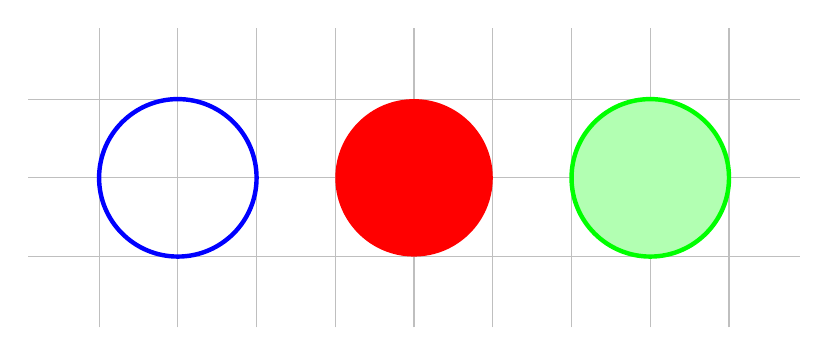
\begin{tikzpicture}
		\draw[lightgray] (-4.9,-1.9) grid (4.9, 1.9);

		\draw[ultra thick, blue] (-3, 0) circle[radius=1];
		\fill[red] (0, 0) circle[radius=1];
		\filldraw[ultra thick, green, fill=green!30] (3, 0) circle[radius=1];
	\end{tikzpicture}
\end{center}

\begin{center}
	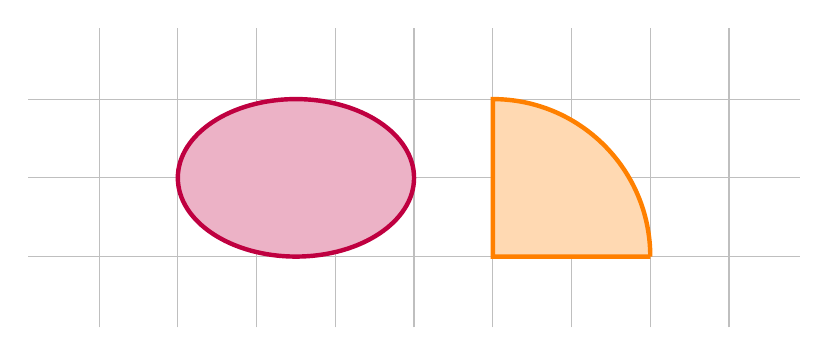
\begin{tikzpicture}
		\draw[lightgray] (-4.9,-1.9) grid (4.9, 1.9);

		\filldraw[ultra thick, purple, fill=purple!30] (-1.5, 0) ellipse (1.5 and 1);

		\filldraw[ultra thick, orange, fill=orange!30] (3, -1) arc(0 : 90 : 2) -- (1, 1) -- (1, -1) -- (3, -1);
	\end{tikzpicture}
\end{center}